\documentclass[10pt,twocolumn,letterpaper]{article}

\usepackage{icb}
\usepackage{times}
\usepackage{epsfig}
\usepackage{graphicx}
\usepackage{amsmath}
\usepackage{amssymb}
\usepackage{eso-pic}

% Include other packages here, before hyperref.

% If you comment hyperref and then uncomment it, you should delete
% egpaper.aux before re-running latex.  (Or just hit 'q' on the first latex
% run, let it finish, and you should be clear).
%\usepackage[pagebackref=true,breaklinks=true,letterpaper=true,colorlinks,bookmarks=false]{hyperref}

\icbfinalcopy % *** Uncomment this line for the final submission

\def\icbPaperID{****} % *** Enter the IJCB Paper ID here
\def\httilde{\mbox{\tt\raisebox{-.5ex}{\symbol{126}}}}

% Pages are numbered in submission mode, and unnumbered in camera-ready
\ificbfinal\pagestyle{empty}\fi
\begin{document}

%%%%%%%%% TITLE
\title{Investigation of muscular architecture in ultrasound images}

\author{Thomas Bergmueller, Martin Schnoell\\
Medical Imaging LAB\\
Master program: Applied Image and Signal Processing\\
Fachhochschule Salzburg\\
%Institution1 address\\
{\tt\small tbergmueller.aise-m2013@fh-salzburg.ac.at, mschnoell.aise-m2013@fh-salzburg.ac.at}
% For a paper whose authors are all at the same institution,
% omit the following lines up until the closing ``}''.
% Additional authors and addresses can be added with ``\and'',
% just like the second author.
% To save space, use either the email address or home page, not both
%\and
%Second Author\\
%Institution2\\
%First line of institution2 address\\
%{\tt\small secondauthor@i2.org}
}

\maketitle
\thispagestyle{empty}

%%%%%%%%% ABSTRACT
\begin{abstract}
   The ABSTRACT is to be in fully-justified italicized text, at the top
   of the left-hand column, below the author and affiliation
   information. Use the word ``Abstract'' as the title, in 12-point
   Times, boldface type, centered relative to the column, initially
   capitalized. The abstract is to be in 10-point, single-spaced type.
   Leave two blank lines after the Abstract, then begin the main text.
   Look at previous ICB abstracts to get a feel for style and length.
\end{abstract}

%%%%%%%%% BODY TEXT

\section{Introduction}
The main goal of this project was to write an algorithm which automatically calculates the angle between the aponeurosis and the muscle fibers of the Vastus Lateralis which is the muscle on the thigh right over the knee. This angle correlates with the constitution of the muscle.
For this project we used ultrasound images.  
Figure \ref{fig:VastusLateralis} shows the location of the Vastus Lateralis and an example ultrasound image in which both aponeuroses (lower and upper one) as well as the line is drawn which represents the muscle fibers (dashed line). Between this muscle fibers and the aponeurosis the angle should be calculated. In the most cases, the two aponeuroses are parallel, so there is no difference between taking the upper or lower one for the calculations. However, sometimes the two aponeuroses are not parallel and then, usually, the lower one is used. 


\begin{figure}
	\begin{center}		
		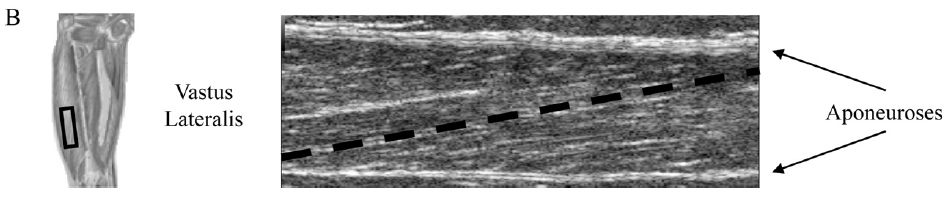
\includegraphics[width=1\linewidth]{img/VastusLateralis}
	\end{center}
	\caption{Vastus Lateralis (left) and an example ultrasound image in which both aponeuroses (lower and upper one) as well as the line is drawn which represents the muscle fibers (dashed line). \cite{NCronin13a}}
	\label{fig:VastusLateralis}
	
\end{figure}

Usually, this angle is calculated manually, by fitting lines to an ultrasound image on the computer and then calculate the angle by hand.

The available groundtruth consists of 22 ultrasound images of the Vastus Lateralis from 12 different patients.
Figure \ref{fig:im1_orig} shows one original image of the dataset.

\begin{figure}
	\begin{center}		
		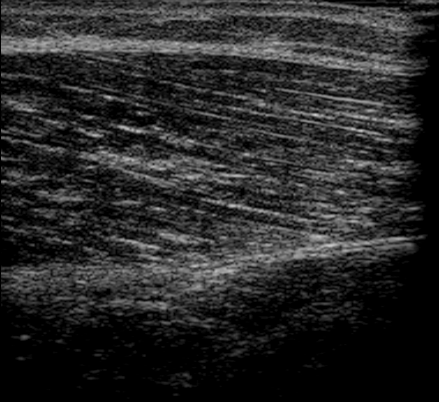
\includegraphics[width=1\linewidth]{img/im1_original}
	\end{center}
	\caption{One original image of the dataset.}
	\label{fig:im1_orig}
	
\end{figure}

For every image two or three different measurements of the angle exist, which partly vary significantly. For example, is the biggest difference of two measurements for the same image (!) 5.7 degree (image with ID 1). In the most cases, however, the single measurements are in the range of +/- 1.5 to the mean.
For our implementation we calculated the mean angle of all measurements from one image and took this mean angle as a reference.

\section{Proposed algorithms}
We worked on two different algorithms in order to determine the angle. The first one is the Hough transform, which is a well-known algorithm for detecting lines in an image. The second one is based on template matching. ...Here, one patch is determined and shifted over the images, looking for matches...

\subsection{Hough transform}
The Hough transform is a well-known and established algorithm for detecting lines and other shapes in images. For the implementation, we used MATLAB R2013a and the inbuilt MATLAB function hough.
This are the main steps of our implementation:

\begin{enumerate}
     \item Gamma correction for enhancing the white pixels
     \item Binarization of the image
     \item Hough transform applied directly on the binary image in order to detect the aponeurosis (the most prominent line)
     \item Canny edge detection on the binary image
     \item Hough transform on the edge image
     \item Finally: Calculate the mean angle of all muscle fiber candidates and then determine the difference between the angle of the aponeurosis and the mean. This results in the final angle
\end{enumerate}

For detecting the aponeurosis (step 3) we also restricted the hough function to only search for lines which are nearly horizontal ( +/- 10 degree roughly). This increases the probability for finding the correct aponeurosis. In step 6, finding the muscle fiber candidates means that the 25 most prominent lines are used. Here, the angle is also restricted to the range from ~6 to ~30 degree since almost all muscle fibers in the groundtruth are in this range and lines with other angles are then clearly outliers. Furthermore, depending on the position of the aponeurosis (at the top or bottom), the fiber candidates have to clearly also lay below (detected aponeurosis is at the top) or above (apo. at bottom) the aponeurosis.

Figure \ref{fig:im1_hough_apo} shows the detected aponeurosis and \ref{fig:im1_hough_fibers} shows the muscle fiber candidates on the image with ID 1 of the database.

\begin{figure}
	\begin{center}		
		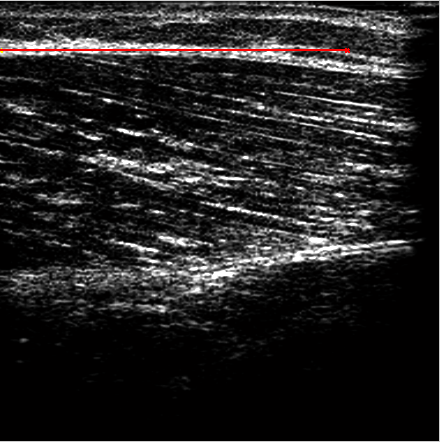
\includegraphics[width=1\linewidth]{img/im1_hough_apo}
	\end{center}
	\caption{This image shows the detected aponeurosis (red line) of the hough transform approach.}
	\label{fig:im1_hough_apo}
	
\end{figure}

\begin{figure}
	\begin{center}		
		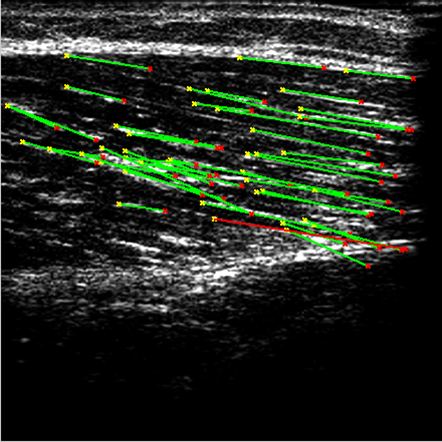
\includegraphics[width=1\linewidth]{img/im1_hough_fibers}
	\end{center}
	\caption{This image shows the 25 detected muscle fiber candidates from which the mean angle is taken.}
	\label{fig:im1_hough_fibers}
	
\end{figure}

\subsection{Template Matching}
...

\section{Results}
The average error/distance for all 22 images of both approaches: Hough transform: 2.48 degree. Template matching: 3.06 degree.

Figure \ref{fig:errorPlot} shows the error plot of both algorithms.

\begin{table}
\begin{center}
\begin{tabular}{| l | l | l | l |}
  \hline
  \emph{Image ID} & \emph{GT} & \emph{HT} & \emph{TM} \\ \hline
  1 & 13.73 & 12.82 & 18.43 \\ \hline
  2 & 16.07 & 13.39 & 17.24 \\ \hline
  3 & 11.70 & 13.34 & 10.56 \\ \hline
  4 & 12.00 & 13.53 & 11.50 \\ \hline
  5 & 13.55 & 10.64 & 7.10 \\ \hline
  6 & 11.60 & 14 & -666 \\ \hline
  7 & 17.20 & 11.34 & 16.83 \\ \hline
  8 & 10.63 & 12.27 & 12.32 \\ \hline
  9 & 11.17 & 11.16 & 8.49 \\ \hline
  10 & 16.47 & 10.86 & 11.19 \\ \hline
  11 & 12.10 & 11.93 & 15.12 \\ \hline
  12 & 13.35 & 13.56 & 11.90 \\ \hline
  13 & 13.57 & 15.09 & 11.65 \\ \hline
  14 & 19.50 & 14.67 & 20.56 \\ \hline
  15 & 24.90 & 14.57 & 17.35 \\ \hline
  16 & 13.23 & 12.87 & 9.59 \\ \hline
  17 & 14.20 & 12.57 & 12.90 \\ \hline
  18 & 13.75 & 12.66 & 9.03 \\ \hline
  19 & 17.30 & 13.83 & 9.42 \\ \hline
  20 & 17.97 & 14.66 & 11.63 \\ \hline
  21 & 10.37 & 11.73 & 9.51 \\ \hline
  22 & 12.30 & 11.19 & 13.49 \\ \hline
\end{tabular}
\caption{Comparison of the angles from the groundtruth (GT), the hough transform approach (GT) and from the template matching approach (TM).}
\label{tab:results}
\end{center}
\end{table}

\begin{figure}
	\begin{center}		
		\includegraphics[width=1\linewidth]{img/errorPlot2}
	\end{center}
	\caption{Error plot of both approaches.}
	\label{fig:errorPlot}
	
\end{figure}

\subsection{Weaknesses of Hough transform}

\subsection{Weaknesses of template matching}

\subsection{Comparison of both approaches}

\section{Conclusion}
There are images where the automatic angle calculation works well, but there are also images were it doesn't work so well...

{\small
\bibliographystyle{ieee}
\bibliography{egbib}
}

\end{document}
